% siminos/atlas/chart.tex  pdflatex atlas
% $Author$ $Date$

\section{Charting the \reducedsp: Global atlas}
\label{s:chart}

    \ifdraft\color{blue}
    \begin{itemize}
      \item flow in a \slice: \cLf\ example
      \item {\chartBord}: \cLf\ example
      \item 2-chart atlas, ridges:  \cLf\ example

      \item gauge fixing, geometric phase?
    \end{itemize}
    \color{black}\fi


%%%%%%%%%%%%%%%%%%%%%%%%%%%%%%%%%%%%%%%%%%%%%%%%%%%%%%%%%%%%%%%%%%%%%
\begin{figure}
   \centering
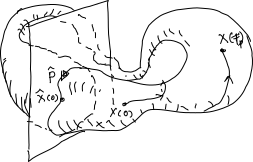
\includegraphics[width=0.40\textwidth]{A29sliceWurst}
   \caption{\label{fig:sliceimage}
Wurst, sliced.
      Every slice hyperplane cuts every group orbit at least twice (see
      \reffig{fig:slice}), once at orbit's closest passage to the
      {\template}, and another time at the most distant passage, also
      satisfying the slice condition \refeq{PCsectQ0}. An $\SOn{2}$ \rpo\
      is topologically a torus, so the two cuts are the two \po\ images
      of the same \rpo, the good close one, and the bad distant one, on
      the other side of {\sliceBord}, and thus not in the slice.
   }
\end{figure}
%%%%%%%%%%%%%%%%%%%%%%%%%%%%%%%%%%%%%%%%%%%%%%%%%%%%%%%%%%%%%%%%%%%%%

%%%%%%%%%%%%%%%%%%%%%%%%%%%%%%%%%%%%%%%%%%%%%%%%%%%%%%%%%%%%%%%%%%%%%%
%\begin{figure}
%   \centering
%  (a)
%~~(b) 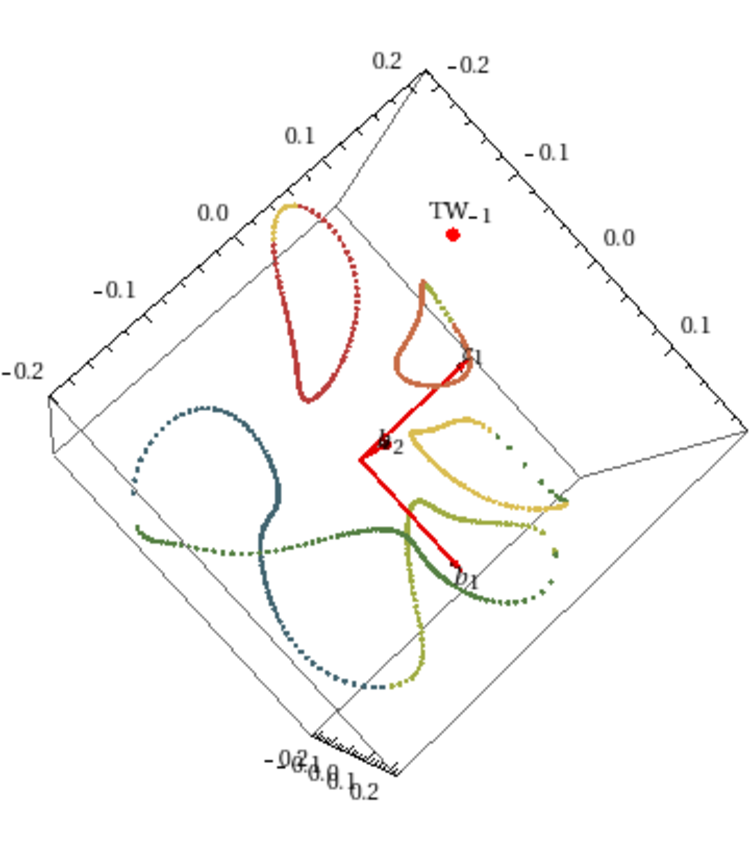
\includegraphics[width=0.45\textwidth]{ks22rpo16mfAll}
%   \caption{ \label{ks22rpo16mf}
%(color online)
%\KS\ \rpo\ with $\period{p}=16.31$, $\shift_p=-2.863$ in a \slice\
%fixed by a \reqv\ \slicep.
%(a)
%(b)
%All intersections of the 2-torus \rpo\ with the \slice\ are plotted.
%Color-coding represents internal numbering of solutions and changes along
%orbits when the number of solutions for $\theta$ changes. We have $3$
%closed-loop images of the \rpo\ and $3$ images that appear to connect to
%a closed loop (from \cite{SiminosThesis}).
%}
%\end{figure}
%%%%%%%%%%%%%%%%%%%%%%%%%%%%%%%%%%%%%%%%%%%%%%%%%%%%%%%%%%%%%%%%%%%%%%

%%%%%%%%%%%%%%%%%%%%%%%%%%%%%%%%%%%%%%%%%%%%%%%%%%%%%%%%%%%%%%%%
 %% chartBord-m*.* replaces FrCv11.tex inflectHype.*
 \begin{figure}
 \begin{center}
  \setlength{\unitlength}{0.30\textwidth}
  %% \unitlength = units used in the Picture Environment
(a)
  \begin{picture}(1,0.91596465)%
    \put(0,0){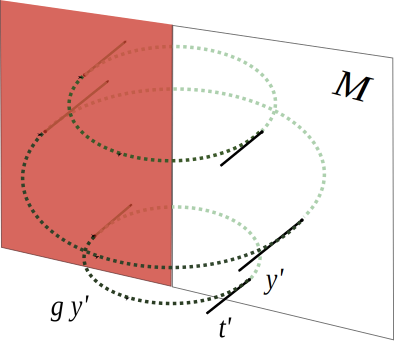
\includegraphics[width=\unitlength]{chartBord-m1}}%
    \put(0.84045332,0.67950567){\color[rgb]{0,0,0}\makebox(0,0)[lb]{\smash{$\pSRed$}}}%
    \put(0.12835189,0.11720037){\color[rgb]{0,0,0}\makebox(0,0)[lb]{\smash{$\LieEl\slicep$}}}%
    \put(0.67299795,0.18547195){\color[rgb]{0,0,0}\makebox(0,0)[lb]{\smash{$\slicep$}}}%
    \put(0.55341875,0.06171734){\color[rgb]{0,0,0}\makebox(0,0)[lb]{\smash{$\sliceTan{}$}}}%
  \end{picture}%
\\
(b)
  \begin{picture}(1,0.91727402)%
    \put(0,0){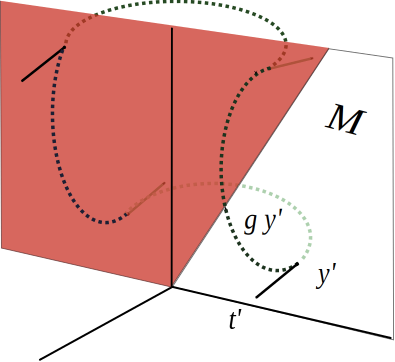
\includegraphics[width=\unitlength]{chartBord-m2}}%
    \put(0.82257887,0.59549577){\color[rgb]{0,0,0}\makebox(0,0)[lb]{\smash{$\pSRed$}}}%
    \put(0.80526889,0.1997715){\color[rgb]{0,0,0}\makebox(0,0)[lb]{\smash{$\slicep$}}}%
    \put(0.57844296,0.0831667){\color[rgb]{0,0,0}\makebox(0,0)[lb]{\smash{$\sliceTan{}$}}}%
    \put(0.61811177,0.33705605){\color[rgb]{0,0,0}\makebox(0,0)[lb]{\smash{$\LieEl\slicep$}}}%
  \end{picture}%
 \end{center}
 \caption{\label{fig:chartBord}  %fig:slice}
\ChartBord: For $\SOn{2}$ two hyperplanes are associated with  a given
{\template} \slicep; the slice $\pSRed$, and the hyperplane of points
$\sspSing$ normal to \refeq{sliceSingl0}, the quadratic Casimir-weighted
vector $\Lg^2\slicep$. The intersection of the two hyperplanes is the
$(d\!-\!2)$\dmn\ hyperplane {\em \chartBord} $\sspRSing \in S$, within
which all group tangents $\groupTan(\sspRSing)$ lie in the slice and are
thus normal to $\sliceTan{}$. Beyond this boundary, the group orbits
pierce the \slice\ hyperplane in the wrong direction, so only the
half-hyperplane that contains the \template\ belongs to the slice. The
{\chartBord} is not easy to visualize; For the lack of dimensions, here
it is drawn here as a `line,' the $z$ axis in this 3\dmn\ sketch. (a) If
the equivariant coordinates transform only under the $m=1$ representation
of $\SOn{2}$, every group orbit is a circle, and crosses the  \slice\
hyperplane twice. However, if there are coordinates that transform as
higher $m$, group orbit can pierce the hyperplane up to $2m$ times, and
the {\chartBord} lies closer to the template. (b) For example, a group
orbit for a combination of $m=1$ and $m=2$ equivariant coordinates
resembles a baseball seam, and can be sliced 4 times, out of which only
the point closest to the \template\ is in the slice (from \wwwcb{}).
 }%
 \end{figure}
%%%%%%%%%%%%%%%%%%%%%%%%%%%%%%%%%%%%%%%%%%%%%%%%%%%%%%%%%%%%%%%%


%%%%%%%%%%%%%%%%%%%%%%%%%%%%%%%%%%%%%%%%%%%%%%%%%%%%%%%%%%%%%%%%
%% A29-2tmplts.* A29-2tmplSl.*
%% Predrag 2012-03-20: see dasbuch/book/FigSrc/inkscape/00ReadMe.txt
%% remember to insert A29-2slices.eps into ChaosBook
 \begin{figure}
 \begin{center}
  \setlength{\unitlength}{0.30\textwidth}
  %% \unitlength = units used in the Picture Environment
(a)\;\;
  \begin{picture}(1,0.92174023)%
    \put(0,0){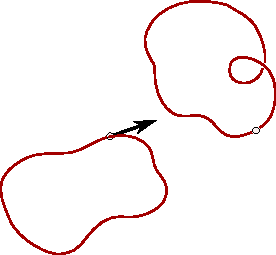
\includegraphics[width=\unitlength]{A29-2tmplts}}%
    \put(0.38186388,0.34995272){\color[rgb]{0,0,0}\makebox(0,0)[lb]{\smash{$\slicep{}^{(1)}$}}}%
    \put(0.41769945,0.50079738){\color[rgb]{0,0,0}\makebox(0,0)[lb]{\smash{$\sliceTan{}{}^{(1)}$}}}%
    \put(0.87339467,0.35886318){\color[rgb]{0,0,0}\makebox(0,0)[lb]{\smash{$\ssp'{}^{(2)}$}}}%
  \end{picture}%
\\
(b)\;\;
  \begin{picture}(1,1.14107266)%
    \put(0,0){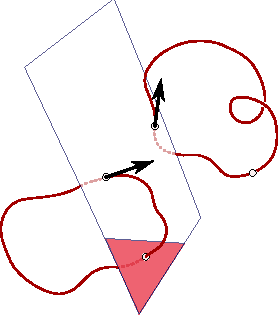
\includegraphics[width=\unitlength]{A29-2tmplSl}}%
    \put(0.54442322,0.48851386){\color[rgb]{0,0,0}\makebox(0,0)[lb]{\smash{$\sliceTan{}{}^{(1)}$}}}%
    \put(0.33649368,0.41474621){\color[rgb]{0,0,0}\makebox(0,0)[lb]{\smash{$\slicep{}^{(1)}$}}}%
    \put(0.41644523,0.62981493){\color[rgb]{0,0,0}\makebox(0,0)[lb]{\smash{$\slicep{}^{(2)}$}}}%
    \put(0.616644,0.84680609){\color[rgb]{0,0,0}\makebox(0,0)[lb]{\smash{$\sliceTan{}{}^{(2)}$}}}%
    \put(0.88017597,0.4261647){\color[rgb]{0,0,0}\makebox(0,0)[lb]{\smash{$\ssp'{}^{(2)}$}}}%
    \put(0.29194797,0.95658666){\color[rgb]{0,0,0}\makebox(0,0)[lb]{\smash{$\pSRed{}^{(1)}$}}}%
  \end{picture}%
 \end{center}
 \caption{\label{fig:A29-2tmplts}
A 2-chart atlas. Sketch
    (a)
depicts two templates $\slicep{}^{(1)}$, $\ssp'{}^{(2)}$, each with its
group orbit. Start with the {\template} $\slicep{}^{(1)}$. All group
orbits traverse its $(d\!-\!1)$\dmn\ slice hyperplane, including the
group orbit of the second {\template} $\ssp'{}^{(2)}$.
    (b)
Replace the second
{\template} by its closest group-orbit point $\slicep{}^{(2)}$, \ie, the
point in \slice\ $\pSRed{}^{(1)}$. This is allowed as long as  $\slicep{}^{(2)}$ is
closer than the $\pSRed{}^{(1)}$ {\chartBord} (red region), otherwise an interpolating,
closer template needs to be introduced.
(from \wwwcb{}).
 }
 \end{figure}
%%%%%%%%%%%%%%%%%%%%%%%%%%%%%%%%%%%%%%%%%%%%%%%%%%%%%%%%%%%%%%%%


%%%%%%%%%%%%%%%%%%%%%%%%%%%%%%%%%%%%%%%%%%%%%%%%%%%%%%%%%%%%%%%%
%% A29-2slices.* A29-2charts.*
%% Predrag 2012-03-20: see dasbuch/book/FigSrc/inkscape/00ReadMe.txt
%% remember to insert A29-2slices.eps into ChaosBook
 \begin{figure}
 \begin{center}
  \setlength{\unitlength}{0.40\textwidth}
  %% \unitlength = units used in the Picture Environment
(c)\;\;
  \begin{picture}(1,0.86567815)%
    \put(0,0){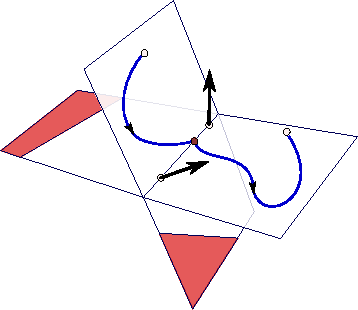
\includegraphics[width=\unitlength]{A29-2slices}}%
    \put(0.3850416,0.38725438){\color[rgb]{0,0,0}\makebox(0,0)[lb]{\smash{$\slicep{}^{(1)}$}}}%
    \put(0.60194012,0.48012421){\color[rgb]{0,0,0}\makebox(0,0)[lb]{\smash{$\slicep{}^{(2)}$}}}%
    \put(0.4042968,0.74412842){\color[rgb]{0,0,0}\makebox(0,0)[lb]{\smash{$\sspRed(0)$}}}%
    \put(0.79647438,0.54627847){\color[rgb]{0,0,0}\makebox(0,0)[lb]{\smash{$\sspRed(\zeit)$}}}%
  \end{picture}%
\\
(d)\;\;
  \begin{picture}(1,0.5127804)%
    \put(0,0){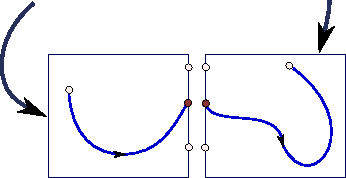
\includegraphics[width=\unitlength]{A29-2charts}}%
    \put(0.16199231,0.03841546){\color[rgb]{0,0,0}\makebox(0,0)[lb]{\smash{$\pSRed{}^{(1)}$}}}%
    \put(0.63051777,0.0374085){\color[rgb]{0,0,0}\makebox(0,0)[lb]{\smash{$\pSRed{}^{(2)}$}}}%
    \put(0.21517269,0.28787637){\color[rgb]{0,0,0}\makebox(0,0)[lb]{\smash{$\sspRed(0)$}}}%
    \put(0.75921701,0.25014044){\color[rgb]{0,0,0}\makebox(0,0)[lb]{\smash{$\sspRed(\zeit)$}}}%
    \put(0.60952792,0.26511997){\color[rgb]{0,0,0}\makebox(0,0)[lb]{\smash{$\slicep{}^{(2)}$}}}%
    \put(0.45827029,0.02997228){\color[rgb]{0,0,0}\makebox(0,0)[lb]{\smash{$\slicep{}^{(1)}$}}}%
  \end{picture}%
 \end{center}
 \caption{\label{fig:A29-2slices}
A 2-chart atlas.
    (c)
Now that the group orbits have been reduced to points, erase them and
consider the two slices through the two {\template s}. As these two
{\template s} are the closest points viewed from either group orbit, they
lie in both \slice s. However, the two tangent vectors
$\sliceTan{}{}^{(1)}$ and $\sliceTan{}{}^{(2)}$ have different
orientations, so they define two distinct \slice\ hyperplanes
$\pSRed{}^{(1)}$ and $\pSRed{}^{(2)}$ which intersect in the
\emph{ridge}, a hyperplane of dimension $(d\!-\!2)$ (here drawn as a
`line,' and in \reffig{fig:A29-1ridge} as intersection of two `volumes')
shared by the template pair that satisfies both \slice\ conditions
\refeq{ridge}. The chart for the neighborhood of each template (a page of
the atlas in part (d)) extends only as far as this ridge. If the
templates are sufficiently close, the {\chartBord} of each \slice\ (red
region) is beyond this ridge, and not encountered by the symmetry-reduced
trajectory $\sspRed(\zeit)$. The reduced trajectory is continuous in the
slice comprised of such charts - it switches the chart whenever it
crosses a ridge.
    (d)
The slice (unique point for each group orbit) is now covered by an atlas
consisting of $(d\!-\!1)$\dmn\ charts $\pSRed{}^{(1)}, \pSRed{}^{(2)},
\cdots$
(from \wwwcb{}).
 }
 \end{figure}
%%%%%%%%%%%%%%%%%%%%%%%%%%%%%%%%%%%%%%%%%%%%%%%%%%%%%%%%%%%%%%%%

%%%%%%%%%%%%%%%%%%%%%%%%%%%%%%%%%%%%%%%%%%%%%%%%%%%%%%%%%%%%%%%%
%% A29-1ridge.*
%% Predrag 2012-03-30: see dasbuch/book/FigSrc/inkscape/00ReadMe.txt
%% remember to insert A29-1ridge.eps into ChaosBook
 \begin{figure}
 \begin{center}
  \setlength{\unitlength}{0.40\textwidth}
  %% \unitlength = units used in the Picture Environment
  \begin{picture}(1,0.89907101)%
    \put(0,0){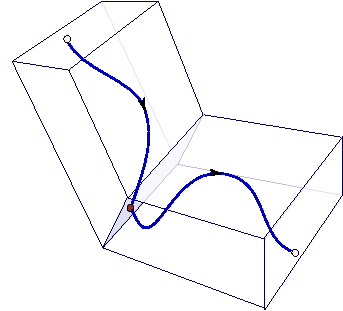
\includegraphics[width=\unitlength]{A29-1ridge}}%
    \put(0.00894598,0.81885604){\color[rgb]{0,0,0}\makebox(0,0)[lb]{\smash{$\sspRed(0)$}}}%
    \put(0.88743345,0.05105926){\color[rgb]{0,0,0}\makebox(0,0)[lb]{\smash{$\sspRed(\zeit)$}}}%
    \put(0.78614059,0.43443027){\color[rgb]{0,0,0}\rotatebox{-25.76142111}{\makebox(0,0)[lb]{\smash{$\pSRed{}^{(1)}$}}}}%
    \put(0.37048948,0.79485578){\color[rgb]{0,0,0}\rotatebox{-61.41291822}{\makebox(0,0)[lb]{\smash{$\pSRed{}^{(2)}$}}}}%
    \put(0.2429401,0.27697318){\color[rgb]{0,0,0}\makebox(0,0)[lb]{\smash{$\sspRed^*_2$}}}%
    \put(0.47832196,0.33514069){\color[rgb]{0,0,0}\makebox(0,0)[lb]{\smash{$\sspRed^*_1$}}}%
  \end{picture}%
 \end{center}
 \caption{\label{fig:A29-1ridge}
The shaded hyperplane is a `blowup' of the ridge in
\reffig{fig:A29-2slices}\,({\it c}). This $(d\!-\!2)$\dmn\ hyperplane
cuts across the symmetry-reduced trajectory $\sspRed(\zeit)$ and thus
serves as a Poincar\'e section that captures dynamics of transits from
the neighborhood of {\template} $\slicep{}^{(1)}$ to the next
neighborhood, {\template} $\slicep{}^{(2)}$. Poincar\'e section transits
are oriented, so $\sspRed^*_1$ and $\sspRed^*_2$ are in the section, but
the third point is not.
(from \wwwcb{}).
 }
 \end{figure}
%%%%%%%%%%%%%%%%%%%%%%%%%%%%%%%%%%%%%%%%%%%%%%%%%%%%%%%%%%%%%%%%

    \PC{
    continue the trajectory in \reffig{fig:A29-1ridge} back through the shaded hyperplane
    Poincar\'e section to emphasize that only one orientation of the
    ridge crossing is counted.
    }
A \slice\ hyperplane captures neighboring group orbits until,
for a point $\sspRSing$ not so close to the \template, its group tangent vector
lies in the \slice,
% \(\braket{\groupTan(\sspRSing)}{\sliceTan{}}= 0 \,,\)
and its group orbit is grazed tangentially rather than sliced
transversally, much like what happens at the \poincBord\
\refeq{eq:sspRSing} for evolution in time. The {\phaseVel}
$\dot{\gSpace}(\sspRSing)$ in \refeq{reconstrEq} then diverges. This is
also a linear condition, and it defines the {\sliceBord} $S$, a
hyperplane in which both points $\sspRSing$ and their group tangents
$\groupTan(\sspRSing)$ lie in the {\slice}\rf{FrCv11},
    %$(d\!-\!2)$\dmn\
    \PC{add Froehlich figure of {\SliceBord} $S$?}
    % 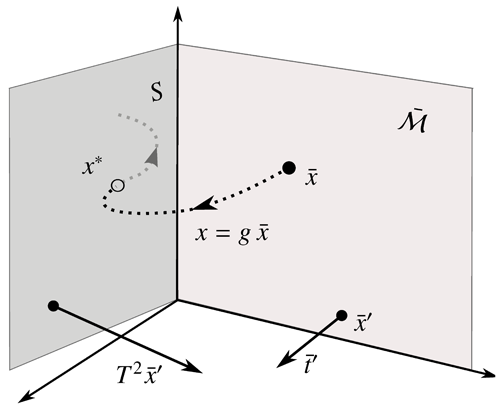
\includegraphics[width=0.80\textwidth]{inflectHype.png}
\beq
\braket{\sspRSing}{\sliceTan{}} \,=\, 0
      \mbox{ and }
\braket{\groupTan(\sspRSing)}{\sliceTan{}} \,=\, 0
\,.
\label{sliceSingl0}
\eeq
A local hyperplane segment of the \slice\ is good only up to the
\sliceBord. The apparent divergence in {\phaseVel} \refeq{reconstrEq} is
a non-physical artifact of the symmetry reduction by tangent hyperplanes,
but a numerical nuisance nevertheless. Here is how we avoid it.

Locally, our initial \slice\ chart $\pSRed{}^{(1)}$ is a ($d\!-\!1$)\dmn\
hyperplane. If we pick another {\template} point $\slicep{}^{(2)}$, it
comes along with its own \slice\ hyperplane $\pSRed{}^{(2)}$. Any
pair of $(d\!-\!1)$\dmn\ local \slice\ hyperplanes intersects
in a `ridge', easy to compute.

\emph{Ridge} {\PoincS} is a segment of hyperplane of dimension
$(d\!-\!2)$ (drawn in \reffig{fig:A29-2slices}\,({\it c}) as a `line' and
in \reffig{fig:A29-1ridge} as intersection of two volumes) shared by a
pair of charts that satisfies both \slice\ conditions \refeq{PCsectQ0},
\beq
\braket{\sspRed^*}{\sliceTan{}{}^{(1)}} = 0
\mbox{ and }
\braket{\sspRed^*}{\sliceTan{}{}^{(2)}} = 0
    \,.
\ee{ridge}

    \KC{2012-03-30}
    {have been thinking about the two chart atlas... \KCedit{I still
    wonder if there is an easier way to do the template choice?} I will
    think about this more }
The rest is geometry of hyperplanes (nothing to do with dynamics, only
with the group theory). In particular, while we motivated slicing by
emphasizing that the choice of templates is where the nonlinear physics
enters, the \slice, \chartBord\ and ridge conditions \refeq{PCsectQ0},
\refeq{eq:chartBord} and \refeq{ridge} are all linear conditions which
depend on the ray defined by the \template\ \slicep, not its magnitude.
Checking whether the {\chartBord} is on the far side of the ridge between
two \slice s is a linear computation, to be undertaken independently of
dynamics; for a symmetry-reduced trajectory moving in $\pSRed{}^{(1)}$
slice one only has to keep checking the sign of
\beq
\braket{\sspRed(\zeit)}{\sliceTan{}{}^{(2)}}
\,.
\ee{eq:chartBord}
Once this changes the sign, the ridge has been crossed, and from then on
the trajectory should be reduced to the $\pSRed{}^{(2)}$ slice. There is
no need to pinpoint this crossing accurately, as long $\sspRed(\zeit)$
stays well clear of all \chartBord s.

Group orbits $\pS_{\slicep}$, group tangents $\groupTan(\slicep)$ and the
associated \slice s are purely group-theoretic, linear concepts: they
know nothing about dynamics. Dynamics enters only through informed
choices of \template s.

The physical task is to, for a given dynamical flow, pick a set of
qualitatively distinct {\template s} (for example, one typical of 2-roll
states, one for 4-roll states, and so on) whose \slice s  are locally
transverse to open sets of nearby orbits, and which together provide a
good global atlas of $\pS/\Group$. Each \slice\ $\pS{}^{(j)}$, provides a
local chart at $\slicep{}^{(j)}$ for a neighborhood of an important,
qualitatively distinct class of solutions. Together they `Voronoi'
tessellate  the curved manifold in which the symmetry-reduced strange
attractor is embedded by a finite set of hyperplane tiles.

%%%%%%%%%%%%%%%%%%%%%%%%%%%%%%%%%%%%%%%%%%%%%%%%%
% 2011-09-09, 2012-03-30 Predrag: add BeThMovFr to
%            continuous.tex overheads, and ChaosBook
% replace A27movFrame*.* everywhere
\begin{figure}
 \begin{center}
(a) 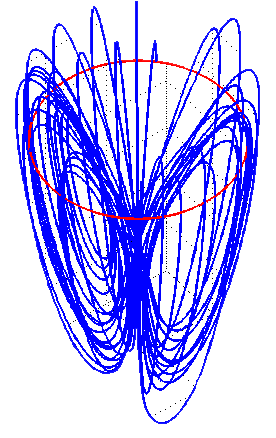
\includegraphics[width=0.20\textwidth]{cLe-fullDB}
~~~~~~
(b) 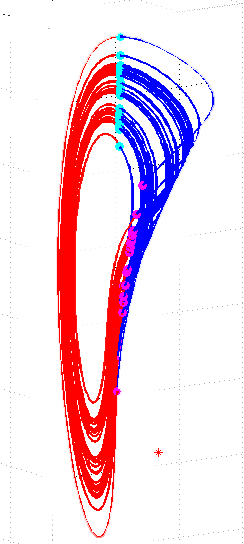
\includegraphics[width=0.16\textwidth]{cLe-2chartsDB}
 \end{center}
  \caption{\label{fig:cLe-2charts}
(a)
Strange attractor of the \cLe\ in the full \statesp.
(b)
The 2-chart atlas (sketched in \reffig{fig:A29-1ridge}) of the strange
attractor of the \cLe, with the ridge Poincar\'e section points
$\sspRed^* \in \PoincS$ marked green (and the wrong direction section
crossings marked purple).
  }
\end{figure}
%%%%%%%%%%%%%%%%%%%%%%%%%%%%%%%%%%%%%%%%%%%%%%%%%%


Thus, in order to chart the \statesp\ of a chaotic flow, a set
of local \slice\ hyperplanes is needed to capture all of the asymptotic
dynamics. The choice of local \slice s should reflect the dynamically
dominant patterns seen in the solutions of nonlinear PDEs. We construct a
global atlas of the dimensionally \reducedsp\ $\pSRed = \pS/\Group$ by
deploying local linear \slice s  $\pS{}^{(j)}$ across neighborhoods of
the qualitatively most important \template\ {\cohStr s}
$\slicep{}^{(j)}$.
    \PC{bring in Lan results\rf{lanCvit07}}

    \ifdraft\color{blue}
``The origin'' or the invariant, fixed-point subspace is a
high-dimensional center space of points not moved by $\Lg_{\theta}$. For
\pCf\ it is the space plumbers prefer to compute in, even though all
turbulence is in the full \statesp. The reason why I really, really want
us to understand what is going on with our atlas in \reffig{fig:A29-2slices}
is that the singularities might be genuine, due to close passages to this
center space, and not taken care of by $\sspRSing$ (which all also
include the `origin'), not just due to bad choice of \template s.
    \color{black}\fi

    \begin{itemize}
      \item an atlas is \emph{not needed} for Newton determination of a
            single orbit; any local section and slice plus time and shift
            constraints is OK, can even move them with each Newton
            iteration. 60,000 \rpo s can be computed\rf{SCD07} this way.
            The question is: what then? and for that you need a good atlas.
    \end{itemize}
